% Section content template for individual Educative lessons
% This file contains the actual content for a specific section
% Generated from Educative API section content

% Section: How Amazon Scales for Prime Day
% Section ID: 4636260997922816
% Section Slug: how-amazon-scales-for-prime-day
% Generated: 2025-12-08T15:50:18.603301

Imagine this: You've been eagerly counting down the days until Amazon Prime Day, waiting to catch that perfect deal. Finally , the moment arrives. You rush to the site... only to face error messages and pages that won't load. Frustrating, right?
\\
This was the reality for millions of shoppers during Amazon's 2018 Prime Day outage. Let 's unpack what actually happened from a System Design perspective

\subsection{Amazon Prime Day outage}\label{m9XdN7krWipTE44SxiLdL}
\\
Amazon experienced a significant outage during its 2018 Prime Day event. The outage lasted for several hours and had a noticeable impact on the shopping experience of millions of customers, as well as on the business itself.
\\
\textbf{Impact:} The main Amazon website and mobile app were affected, with users reporting issues accessing product pages, completing purchases, and loading the home page. According to the \href{https://techcrunch.com/2018/07/18/amazon-prime-day-outage-cost/}{report}, Amazon lost over \$100 million in sales during the downtime, an estimated \$1.2 million per minute.

\begin{figure}[htbp]
 \centering
 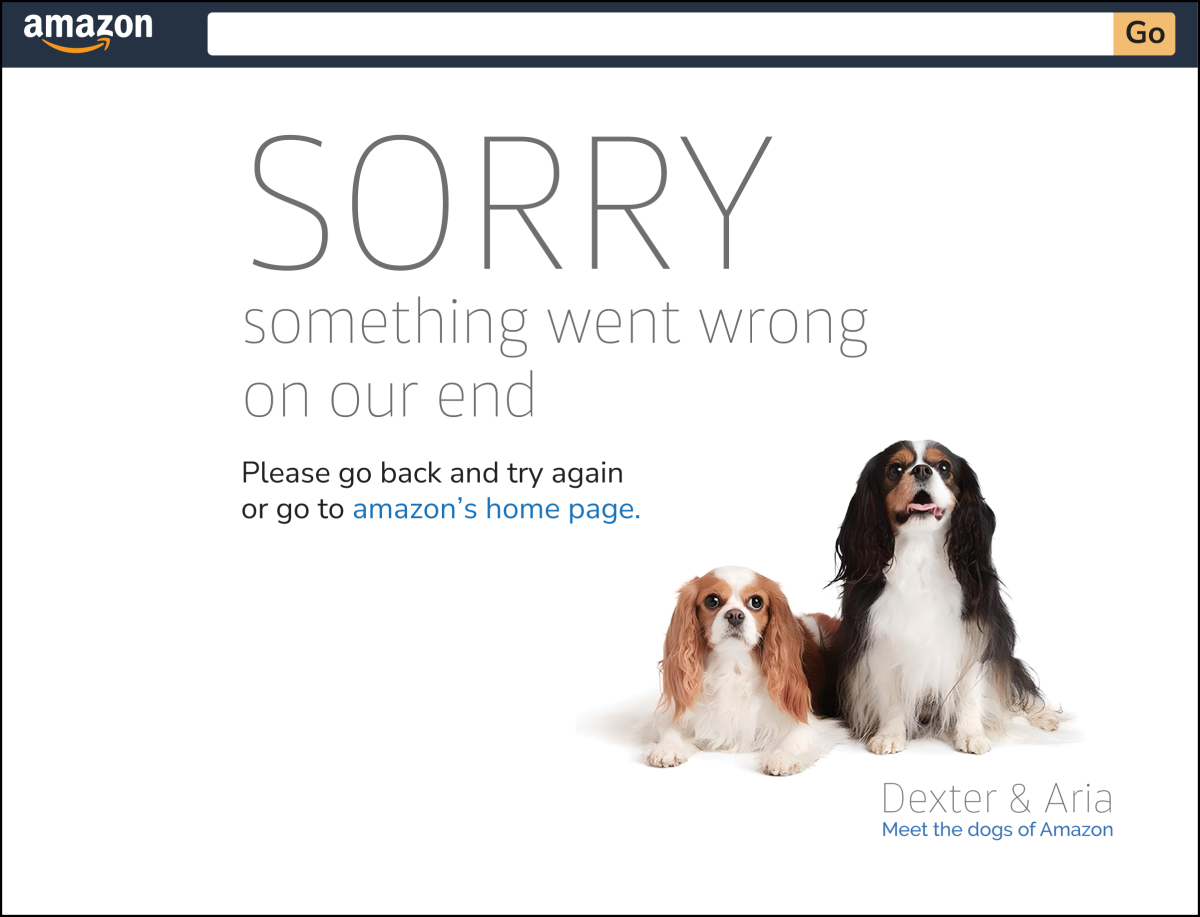
\includegraphics[width=0.15\textwidth]{Images/chapter_45/section_4636260997922816/5493208859148288.png}
 \caption{Amazon's main page on Prime Day 2018}
\end{figure}

\subsubsection{Causes of the outage}\label{AqHZztUJRio9vs8h_BoB4}
\\
While Amazon has not disclosed all the technical details, we can analyze the causes with industry knowledge and engineering principles based on a CNBC report, which includes the following key factors to failure:

\begin{enumerate}
\item
\protect\phantomsection\label{4UecELq6Ffk2MTgdSGMa4}
The first and most important factor is the higher-than-expected spike in traffic, which exceeded Amazon's capacity despite the preparation. This observation is evident from~Amazon's steps, which included falling back to a simpler frontend page and blocking international traffic.
\item
\protect\phantomsection\label{O0-fo5nlNmwd23eEucccn}
Although Amazon employed a robust microservices architecture, it may have faced issues where service dependencies led to cascading failures. This issue was also reported for other Amazon services, including Twitch, Alexa, and Prime Now.
\item
\protect\phantomsection\label{W_BmIL-PtM1q8I-OLUbDG}
While Amazon utilizes autoscaling to handle surges in traffic, delays occurred in scaling up resources due to configuration issues with Amazon's systems and services. This forced Amazon to manually deploy servers to meet the traffic load, which cost time and money.
\end{enumerate}
\\
The CNBC report indicates that the surge in traffic was one of the primary factors Amazon couldn't handle, as it made the service unavailable. The system received approximately 63.5 million requests per second on its storage and computational service (Sable).
\\
In this blog, I'll explore the technical intricacies of scaling for traffic during high-demand periods, using Amazon as our case study.
\\
We'll break down the strategies and approaches that ensure a smooth service, regardless of the number of people searching for products, clicking ``add to cart'', or placing orders. Whether you're a tech enthusiast, an e-commerce entrepreneur, or just someone who wants to understand what happens behind the scenes during these mega-sale events, this journey into Amazon's world of scalability will be enlightening.
\\
Let's explore the importance of availability bound to scalable systems.

\subsection{Importance of scalability and availability}\label{fZZnVcGAk-_JGlECnOZxD}
\\
Scalability is the secret sauce allowing companies like Amazon to handle massive traffic spikes without breaking a sweat.
\\
It's about having the infrastructure to flexibly expand and contract in response to demand. The 2018 Prime Day outage wasn't just a hiccup; it was a wake-up call that even the best in the business can stumble. But many people don't realize that ensuring scalability isn't just about handling spikes in traffic; it's intrinsically linked to availability.
\\
Let's look at how Amazon processes a user's request.
\\
A single API request, such as purchasing an item or performing a search, is routed to multiple backend services, including inventory, payment, shipping, indexing, and recommendation. Each service must handle part of the request to fulfill it successfully.
\\
When scaling, all these backend services need to be scaled together to manage increased load effectively, as seen in the purchasing and search examples below:

\begin{figure}[htbp]
 \centering
 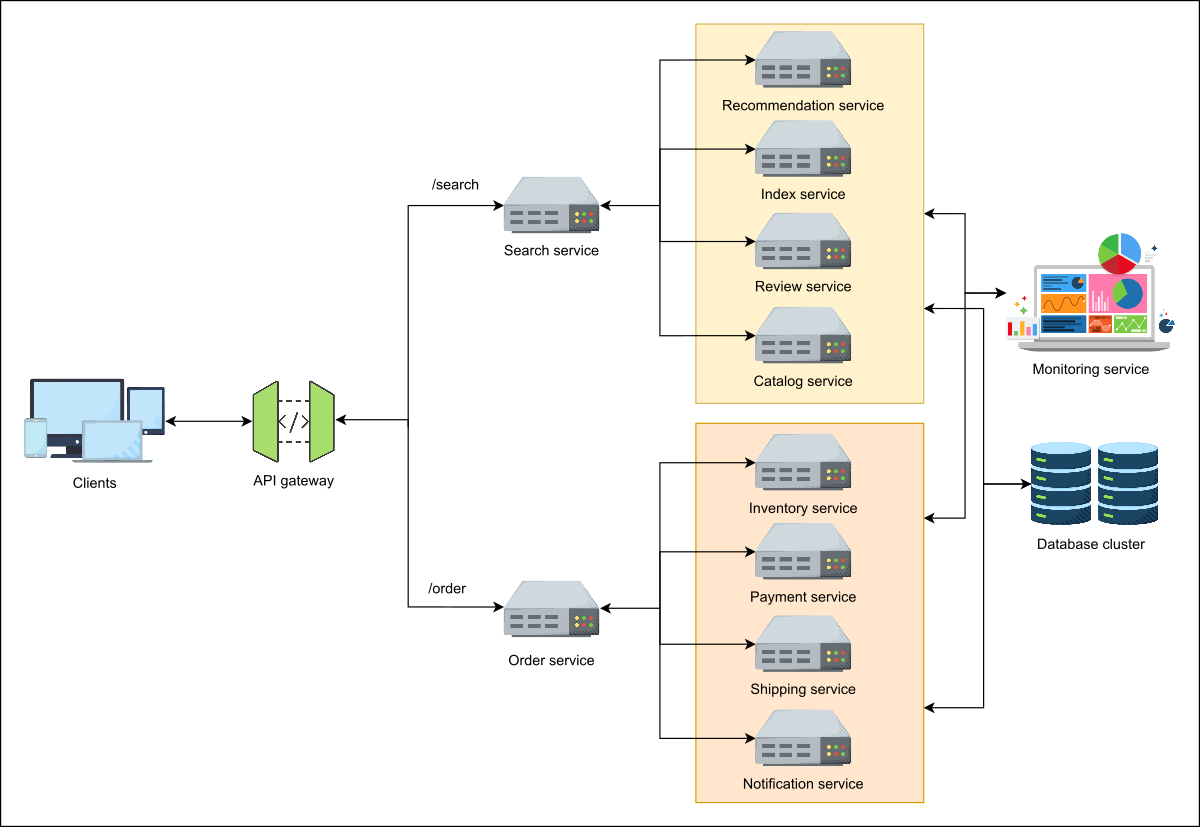
\includegraphics[width=0.5\textwidth]{Images/chapter_45/section_4636260997922816/5662213976752128.png}
 \caption{A depiction of fanning out requests to multiple subservices }
\end{figure}

Availability, keeping the services up and running, is the backbone of any online business. A few minutes of downtime can translate into millions of dollars in lost sales, and a spoiled reputation is additional. Availability is important for the success of a service and a seamless user experience. This means that users can access the service and perform the intended operations at any time. In ~service level agreements (SLAs), availability is defined as a percentage of time, usually represented by 9s, such as \protect\phantomsection\label{katex_inline_3_f08--F6J86r24BoR248}{{{\(99.999 \%\)}}} uptime of the service.
\begin{quote}
\textbf{Note:} When we scale a system to handle a surge in demand, it is also crucial to ensure service availability. No matter how much we scale, if we don't have replicas or failover mechanisms to ensure availability, the service will likely fail, and vice versa.
\end{quote}
\subsubsection{What are the optimal 9s of availability?}\label{D6MMbghEya9v3uB2YCgjw}
\\
When deploying services, an uptime of \protect\phantomsection\label{katex_inline_fS2Drs4038AVLkjC71RJ-}{{{\(99.999 \%\)}}} (five 9s) is assumed as the perfect uptime. This allows for only \protect\phantomsection\label{katex_inline_Btwc7N7UI1-c_K9O9FPwu}{{{\(0.001 \%\)}}} of downtime. Let 's look at some calculations to see~what that entails:

\[
24\ hours \times 365\ days = 8760\ hours/year
\]

\[
8760\ hours \times 60\ minutes = 525600\ minutes/year
\]

\[
525600\ minutes \times \frac{0.001}{100}\ = 5.26\ minutes
\]

A downtime of 0.001\% equals less than 6 minutes; a service will be down for around 6 minutes \emph{in an entire year}. Now , 6 minutes in a year doesn't sound like much, but for services like Amazon, a minute can cost them around a million in sales, especially on events like Prime Day.
\\
Let's estimate Amazon Prime Day\textquotesingle s revenue for 2024 by examining its sales \href{https://capitaloneshopping.com/research/amazon-prime-day-statistics/}{history}. Take a look at the graph below:

\textbf{Amazon Prime Days revenue each year}

\textit{\small [Chart data presented in table format]}

\begin{table}[htbp]
\centering
\small
\adjustbox{max width=\textwidth}{
\begin{tabular}{|p{0.475\textwidth}|p{0.475\textwidth}|}
\hline
\textbf{Year} & \textbf{Revenue (\$ billion)} \\
\hline
\hline
2015 & 0.9 \\
\hline
2016 & 1.45 \\
\hline
2017 & 2.33 \\
\hline
2018 & 4.15 \\
\hline
2019 & 7.16 \\
\hline
2020 & 10.39 \\
\hline
2021 & 11.19 \\
\hline
2022 & 12.09 \\
\hline
2023 & 12.9 \\
\hline
2024 & 14.3 \\
\hline
\end{tabular}
}
\caption{The expected revenue of Amazon in 2024 (in green).}
\label{tab:chart}

\textit{\small Note: Values are in Billion}
\end{table}

\begin{quote}
\textbf{Note:} The expected revenue of Amazon Prime Day 2024 is based on the average annual revenue difference (\$1.43 billion) from the above data.
\end{quote}
\\
Based on the expected revenue for 2024, Amazon is projected to generate approximately \$5 million per minute in sales. Now , let's see how the 9s of availability affect the downtime and, hence, the loss in revenue of Amazon Prime Day:

\textbf{Nines (9s) of availability}

\begin{table}[htbp]
\centering
\small
\adjustbox{max width=\textwidth}{
\begin{tabular}{|p{0.262\textwidth}|p{0.170\textwidth}|p{0.166\textwidth}|p{0.159\textwidth}|p{0.192\textwidth}|}
\hline
\textbf{Availability} & \textbf{Downtime Per Year} & \textbf{Downtime Per Month} & \textbf{Downtime Per Day} & \textbf{Revenue Loss Per Day} \\
\hline
\hline
1 nine ---- 90\% & 36.5 days & 72 hours & 2.4 hours & \$720 million \\
\hline
2 nines ---- 99.0\% & 3.65 days & 7.20 hours & 14.4 minutes & \$72 million \\
\hline
3 nines ---- 99.9\% & 8.76 hours & 43.8 minutes & 1.46 minutes & \$7.3 million \\
\hline
4 nines ---- 99.99\% & 52.56 minutes & 4.32 minutes & 8.64 seconds & \$0.72 million \\
\hline
5 nines ---- 99.999\% & 5.26 minutes & 25.9 seconds & 0.86 seconds & \$0.072 million \\
\hline
\end{tabular}
}
\caption{Nines (9s) of availability}
\end{table}

The above back-of-the-envelope calculations estimate the loss if Amazon faces downtime on the next Prime Day (2024).
\begin{quote}
\textbf{Note:} The problem with achieving five or six nines of availability is that it costs a lot of money and effort. The good thing is that you don't need to have five or six nines of daily availability, except for days like Amazon Prime Day. The cost of achieving five 9s is so high that the returns do not justify the investment.
\end{quote}
\subsubsection{Isn't Amazon Web Services (AWS) good enough?}\label{3eGpJMemu1IXpnV-RpQB3}
\\
Amazon Web Services (AWS), Amazon's cloud platform, offers a powerful suite of services designed to keep modern applications resilient and highly available.
\\
From Amazon EC2 Auto Scaling, which automatically adjusts compute capacity, to Elastic Load Balancing (ELB), which distributes incoming traffic across healthy targets, AWS provides the foundational tools needed to handle massive traffic surges---such as those seen during events like Amazon Prime Day.
\\
However, even the most advanced cloud infrastructure can experience issues.
\\
In many cases, outages occur not because the tools are insufficient, but because of how they are configured, monitored, and managed. AWS services provide the capabilities, but achieving true reliability requires engineering teams to configure those services correctly, establish clear scaling policies, design for failure, and continuously test their systems.
\\
This serves as an important reminder: AWS offers the building blocks, but availability and scalability ultimately depend on sound architectural decisions. To understand how Amazon achieves this at scale, let's examine the core principles behind designing systems for high availability and elastic scalability.

\subsection{An overview of Amazon's e-commerce infrastructure}\label{zJ4qIbdXcpdLXynmqHyT7}
\\
Amazon started as an online bookstore and has since evolved into the world\textquotesingle s largest e-commerce platform, offering a vast array of products.
\\
Let's see how the Amazon e-commerce platform works for selling and purchasing goods. The Amazon system must be highly scalable and available to handle millions of transactions per day, particularly during events like Amazon Prime Day.
\\
Yes, you guessed it right; it should also be performant and consistent, which, for the time being, will be considered secondary metrics. The primary metrics are scalability and availability. Let 's have a walkthrough of the Amazon back-end infrastructure as given in this high-level design:

\begin{figure}[htbp]
 \centering
 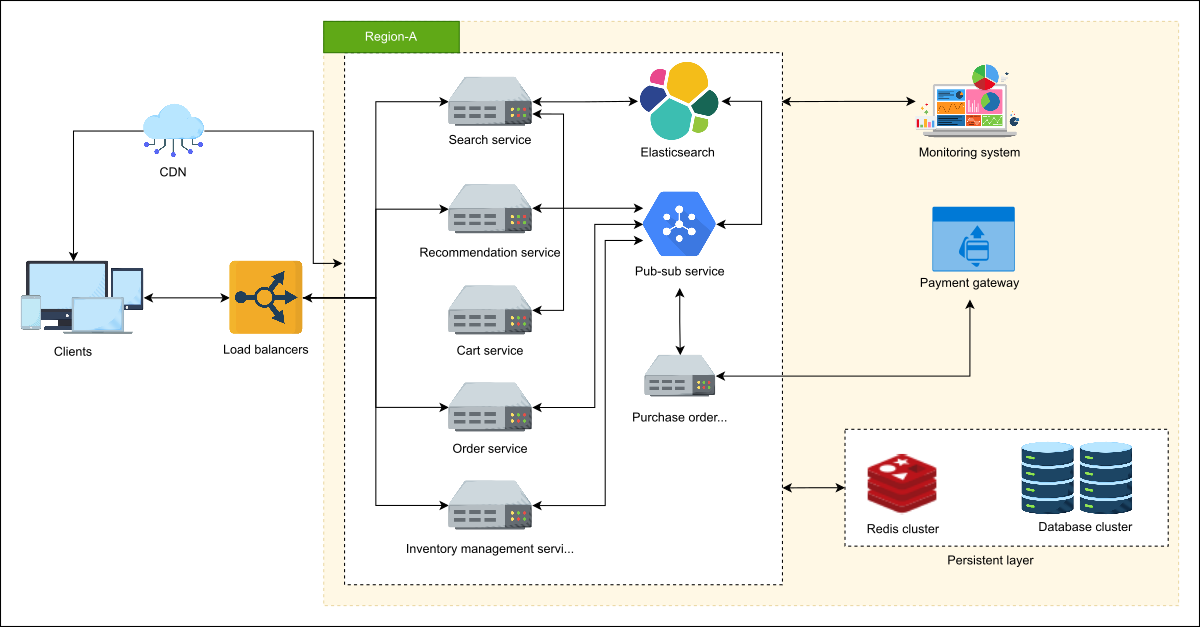
\includegraphics[width=0.5\textwidth]{Images/chapter_45/section_4636260997922816/5211949670989824.png}
 \caption{A high-level design of Amazon’s e-commerce system}
\end{figure}

Initially, the users can visit the homepage to search for an item of interest.
\\
The search service utilizes the Elasticsearch system for several key advantages, including performance, scalability, and full-text search features. At the back of the homepage is a recommendation service that provides personalized recommendations to users based on their purchase history or search activity.
\\
If the user is new, they are shown some trending products on the home page.
\\
Once the users select items and add them to the shopping cart, the cart service is triggered at the backend, which keeps the items in the relevant databases. The order service handles incoming orders from users and stores detailed information about the order, including customer and product information, in the databases.
\\
This service is responsible for capturing the delivery address and the relevant information.
\\
When users attempt to pay and purchase an item, the purchase order is invoked, which interacts with the payment gateway, which, in turn, is responsible for collecting the due amount from the customer's credit card or account. The pub-sub system decouples various services, allowing them to communicate asynchronously.

\subsection{Techniques to ensure scalability and availability}\label{xgBUW0RI0vhNI85bB0lM3}
\\
Let's examine some techniques that can be implemented to ensure the scalability and availability of the system. The most prominent techniques are:

\begin{itemize}
\item
\protect\phantomsection\label{9voLOthFRBNLeAZXEhADI}
\textbf{Database replication, distributed caches, and backups:} Database replication techniques ensure data availability and significantly enhance scalability. Using the right techniques to store and retrieve data is essential to maintaining seamless service continuity. This includes replicating data across multiple databases and regions, partitioning data according to application needs, and maintaining different storage solutions for different data types. Techniques like distributed caching enhance performance by storing frequently accessed data closer to where it is needed, efficiently managing a large volume of incoming requests. Additionally, incorporating regular backups is crucial for disaster recovery. While these strategies require cost and effort, they are essential for maintaining the system's reliability and readiness for unexpected events.
\item
\protect\phantomsection\label{cNFK_-e5G5-4sPxiVrSlq}
\textbf{Load balancing and autoscaling groups:} This is a no-brainer. Impleme\-nting load balancing involves distributing incoming traffic among targets, such as containers, servers, and data ce\-nters. This prevents ove\-rwhelming a single serve\-r and allows another to step in if nee\-ded. Similarly, autoscaling groups enable a system to adjust the number of active instances based on demand, le\-ading to enhanced availability, performance, and user experie\-nce.
\item
\protect\phantomsection\label{R2OExcIB26Oc7dcJoABXV}
\textbf{Redundancy of services:} By duplicating critical services across multiple zones and regions, a system can ensure that even if a service in one region fails, another can take over seamlessly. This redundancy minimizes downtime and latency, handles large requests efficiently, and maintains the platform's reliability, ensuring a consistent user experience.
\item
\protect\phantomsection\label{RykwCeM7ABDAew8G5_eNt}
\textbf{Content Delivery Networks (CDNs):} Utilize CDNs to deliver content to users with low latency and high transfer speeds. By caching content at edge locations worldwide, they ensure that users receive data from the nearest server, reducing load times and improving the overall user experience. It also reduces the burden on the origin servers. CDNs are essential for efficiently handling large amounts of traffic and improving overall availability.
\item
\protect\phantomsection\label{6oAHfhaVSDwW6o7VoNJ0I}
\textbf{Monitoring and auto-recovery mechanisms:} Effective monitoring ensures a system's health and performance. Utilizing tools for real-time monitoring of system metrics (such as response time, resource utilization, access logs, temperature, and security events) and setting up automated alerts helps engineering teams promptly address potential issues. Implementing auto-recovery processes, such as restarting failed instances or triggering automatic failovers, is essential for maintaining service continuity and minimizing downtime. These techniques are vital for proactive system management and ensuring reliable operation under varying conditions.
\item
\protect\phantomsection\label{POZvIVy6-StDBvhMH-ooB}
\textbf{Testing:} Thorough load tests simulating peak traffic conditions are crucial. These tests should account for the worst-case scenarios, ensuring all systems can handle extreme loads.
\end{itemize}
\\
You might think you can get by without the techniques above, and maybe you can, until that one bad day strikes. Being prepared can make all the difference. Trust me, you'll be grateful you invested in these strategies when that day comes.
\\
In reality, ensuring a seamless experience, even on big days, requires considerable engineering brilliance and a commitment to consistent improvement. That 's only the first half of the problem. What happens if there is a failure? That's the second half! You need standby engineering teams on high alert with contingency plan(s) to ensure you recover quickly and successfully.

It is crucial to maintain standby engineering teams that are ready to respond to incidents or system failures at any time. These teams should be equipped with the tools and knowledge to quickly diagnose and resolve issues, ensuring minimal disruption to services. Having dedicated on-call engineers allows the system to maintain high availability and quickly restore services in case of unexpected failures.

Let's see what techniques Amazon uses to ensure scalability and availability in the following table:

\begin{table}[htbp]
\centering
\small
\adjustbox{max width=\textwidth}{
\begin{tabular}{|p{0.267\textwidth}|p{0.683\textwidth}|}
\hline
\textbf{Strategies for Scalability and Availablity} & \textbf{Amazon's Techniques and Services} \\
\hline
\hline
\hfill\break \hfill\break Database replication and backups & \begin{itemize} \tightlist \item \textbf{Amazon RDS} for multi-availability zone deployment \item \textbf{Amazon DynamoDB} for fully managed multiregion, multi-active data replication \item \textbf{Amazon Aurora} for synchronous replication for high availability within a region and asynchronous replication for cross-origin data redundancy \item \textbf{Amazon DocumentDB} for multiprimary replication across multiple availability zones \end{itemize} \\
\hline
Distributed cache & \begin{itemize} \tightlist \item \textbf{Amazon ElasticCache} is the distributed cache solution used for high performance, scalability, and availability \end{itemize} \\
\hline
\hfill\break \hfill\break Load balancing and Autoscaling & \begin{itemize} \tightlist \item \textbf{Amazon Elastic} load \textbf{} balancing for distributing different types of traffic across various services \item \textbf{Amazon EC2} autoscaling for automatically adjusting the number of EC2 instances \item \textbf{Amazon ECS} and \textbf{EKS} autoscaling for containerized applications \end{itemize} \\
\hline
Content Delivery Networks (CDNs) & \begin{itemize} \tightlist \item \textbf{Amazon CloudFront} for placing the content near users \end{itemize} \\
\hline
\hfill\break \hfill\break Monitoring and autorecovery mechanisms & \begin{itemize} \tightlist \item \textbf{Amazon CloudWatch} for monitoring and observing the services \item \textbf{Amazon EC2 Auto Recovery} enables automatic recovery of EC2 instances \item \textbf{AWS Systems Manager} provides a unified user interface for managing AWS resources \item \textbf{AWS Health} provides personalized alerts and recovery guidance in the event of failure \end{itemize} \\
\hline
Testing & \begin{itemize} \tightlist \item \textbf{Amazon GameDay} simulates failures to prepare for unforeseen situations \end{itemize} \\
\hline
\end{tabular}
}
\end{table}

\subsubsection{Key takeaways from the Amazon outage}\label{SWjF181T60gdvRwInKmyW}
\\
Amazon's 2018 Prime Day outage highlights several important lessons for managing high-demand periods for engineering teams and tech enthusiasts:

\begin{itemize}
\item
\protect\phantomsection\label{QeZH9QP3yYycbEX6kHKJH}
Building a perfect system is impossible, but there is nothing wrong with striving to achieve~a well-designed one. How do you achieve that? Keep your design as simple as possible~and evolve it slowly to avoid unnecessary complexities.
\item
\protect\phantomsection\label{dh_R-xcTUsmcY3Uwt0UPN}
Blame the configuration management or load testing teams; systems inevitably fail, even among tech giants like Amazon, Meta, and Google. Surprisingly , if you visit independent services like Downdetector, you may find your favorite application struggling to provide service in some parts of the world. The key aspect here is preparation for such incidents, including mitigation techniques to employ before they occur, a contingency plan in place after they happen, and the lessons learned from past failures.
\item
\protect\phantomsection\label{cCoy_I09xHMJ3Ufc7Bj4E}
Faulty capacity estimation is a primary reason why systems fail. You design systems and prepare for the traffic you estimate. A faulty estimation leads to a faulty design. Therefore, always base your math on meaningful assumptions and intelligent guessesto make informed design decisions.
\end{itemize}

\subsubsection{Conclusion}\label{BjhqMPplxgVRqKm1BR7Xm}
\\
A system like Amazon needs to analyze user behavior and usage patterns and predict traffic spikes.
\\
This can be achieved via advanced analytics, where metrics such as peak viewing times, popular content, and regional user distribution are continuously monitored. Furthermore , traffic patterns can be predicted through big data analytics technology, and the system can be prepared for potential surges.
\\
Simultaneously, monitoring systems can provide valuable insights into current usage and facilitate better resource management.
\\
To handle peak loads effectively, it's essential to introduce autoscaling systems that adjust the number of servers according to demand. AWS utilizes autoscaling groups to automatically add or remove instances based on fluctuations in traffic.
\\
The combination of predictive analytics with reactive scaling and load balancing will enable the system to manage peak loads optimally without sacrificing performance.

% End of section content